\documentclass[12pt]{scrartcl}
\input{NiaLatexHelpers/nia_defs.tex}

\title{\vspace{-2em} Karel the Robot Labs}
\author{}
\date{}

\begin{document}
\maketitle
\vspace{-6em}

\textit{Karel the Robot}, an idea pioneered at Stanford, is a way to teach programming in a visual, entertaining way. Through the four basic commands of \pythonl{move()}, \pythonl{turn_left()}, \pythonl{put_beeper()}, and \pythonl{pick_beeper()}, you will navigate Karel through a series of mazes and learn about coding along the way! There is a Python version of Karel, and that's what we'll use.

\begin{figure}[H]
    \centering
    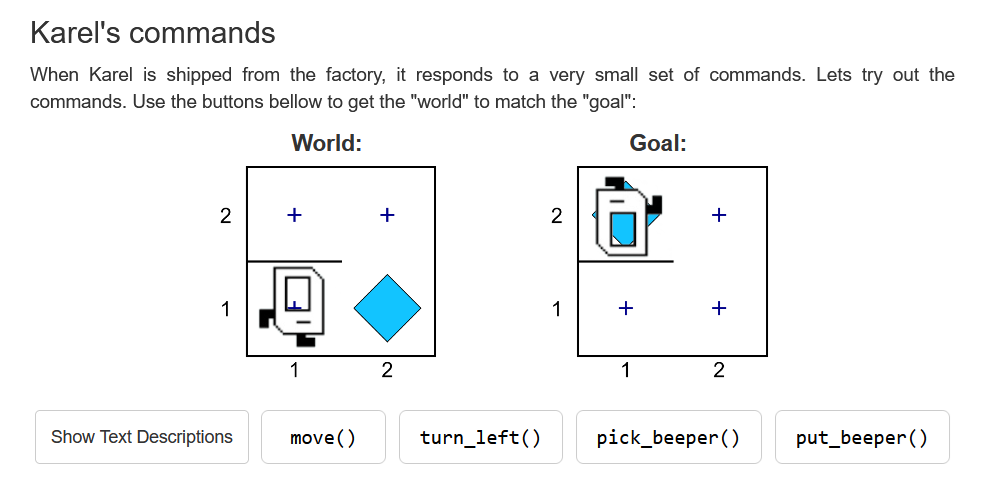
\includegraphics[scale=0.5]{Karel Demonstration.png}
    \caption*{You can try her yourself here: \href{https://compedu.stanford.edu/karel-reader/docs/python/en/chapter1.html}{Link}.}
\end{figure}

\section*{Installation}
Navigate over to \href{https://pypi.org/project/stanfordkarel/#description}{this link} and click on the left sidebar ``Download files.'' From there, you want to download the ``Built Distribution.''

\begin{figure}[H]
    \centering
    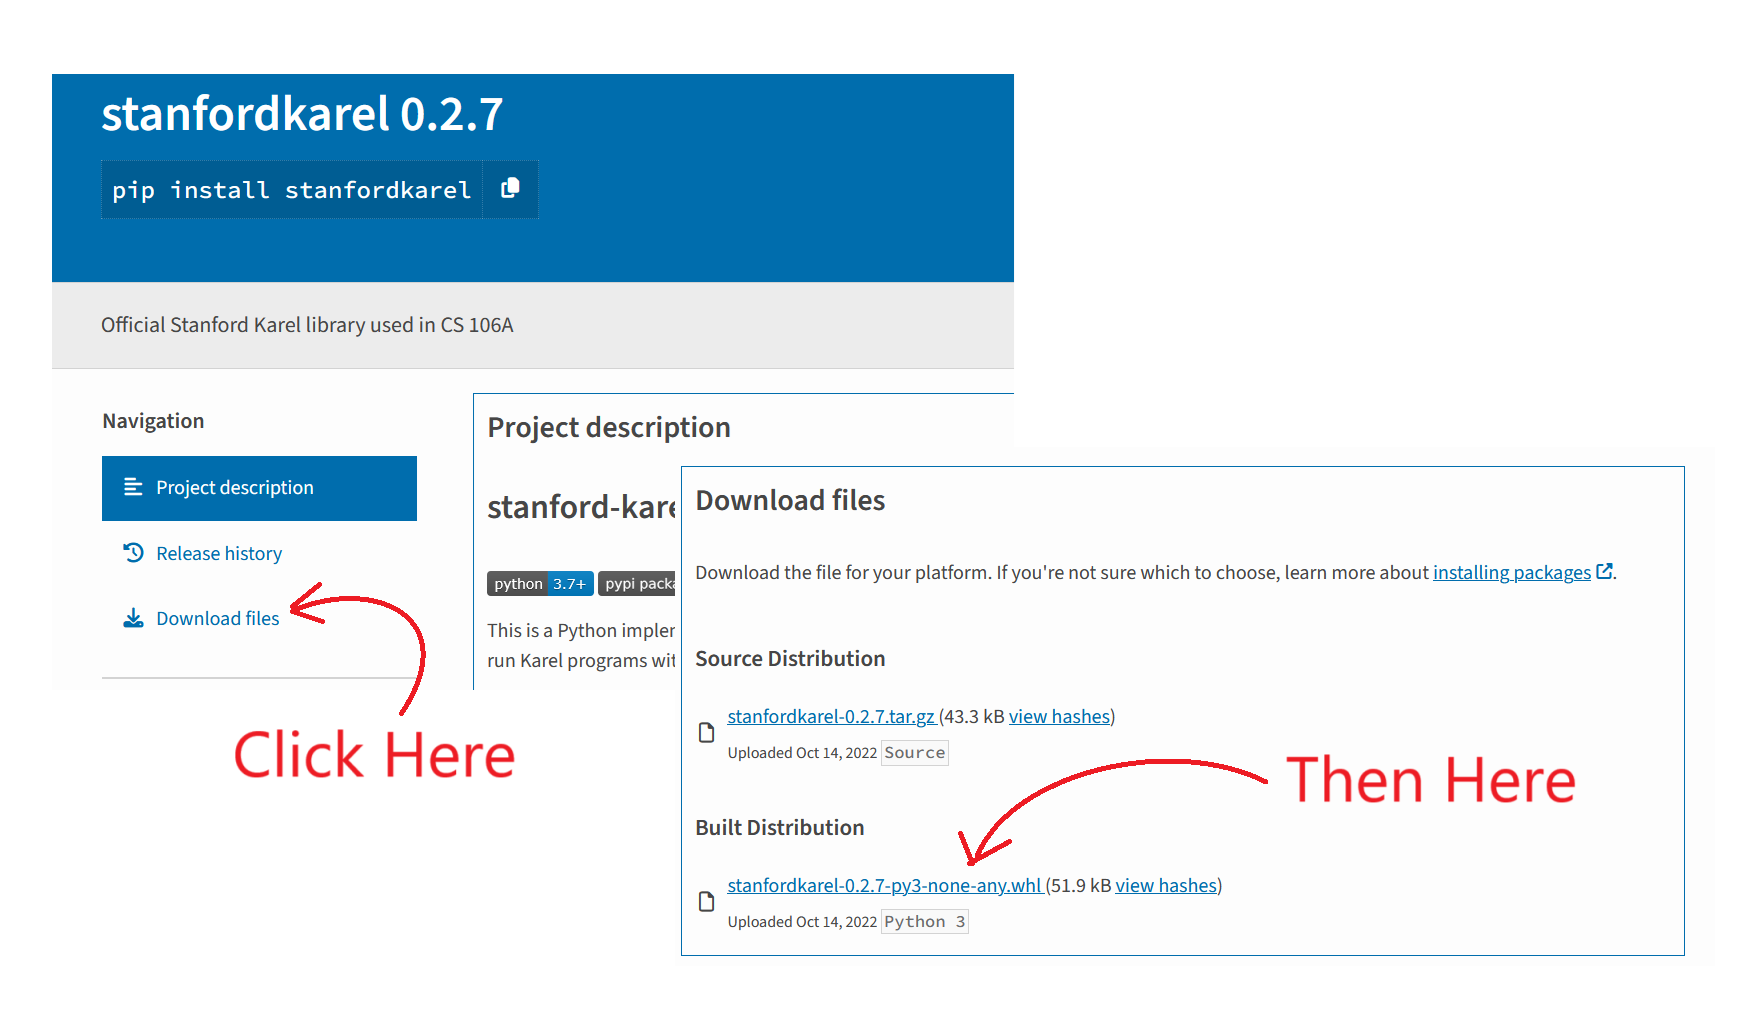
\includegraphics[scale=0.25]{Download It.png}
    \caption*{Karel incoming.}
\end{figure}

Once she's downloaded, double click the file in FileExplorer to start the installation progress. A command prompt window will open up that will install Karel. \textbf{NOTE: Ths may take 30 seconds or longer. Do note close the installation window.}

\begin{figure}[H]
    \centering
    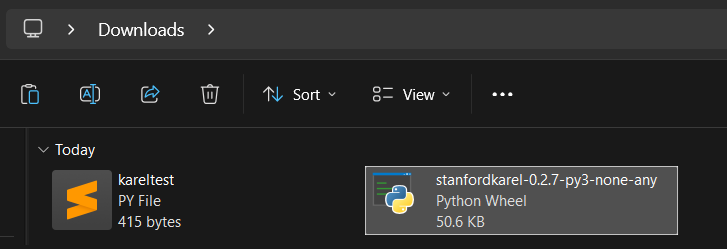
\includegraphics[scale=0.55]{Installation Part 1.png}
    \caption*{My file explorer is in dark mode, so yours may look different.}
\end{figure}

Then, in a new command prompt window, type
\begin{center}
    \codel{python -m pip install stanfordkarel}
\end{center}

Voil\`a! Now Karel will be ready to use.

\begin{figure}[H]
    \centering
    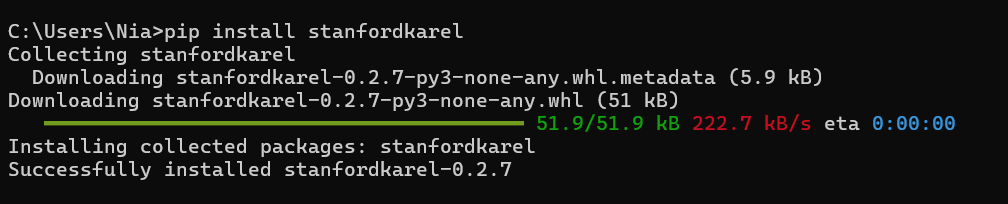
\includegraphics[scale=0.6]{Installation Part 2.png}
    \caption*{Woohoo!}
\end{figure}

If you want to read a tutorial on Karel, you can find it \href{https://compedu.stanford.edu/karel-reader/docs/python/en/chapter1.html}{here}. And \href{https://github.com/TylerYep/stanfordkarel}{this link} has some more information if you scroll down, though it's a bit more techy. But I hope to explain what you need to do in this lab document.

\newpage
\section*{Lab 1: Movement \\
{\small Prerequesties: Functions}
}

In a new python file, copy the following code:
\begin{python}
    from stanfordkarel import *


    def main():
        """Karel code goes here!"""
        turn_left()
        move()
        turn_left()


    if __name__ == "__main__":
        run_karel_program()
\end{python}

There's some code here that uses ideas we do not know yet. The statement \pythonl{from standfordkarel import *} just adds Karel to our file ready to be use. And the code on lines 11 and 12 is a bit beyond our level, but just know that it activates the Karel graphical window that you'll see when you run this code. All you need to worry about is writing Karel code inside \pythonl{main()}!

When you run this code in command prompt, a window will open:

\begin{figure}[H]
    \centering
    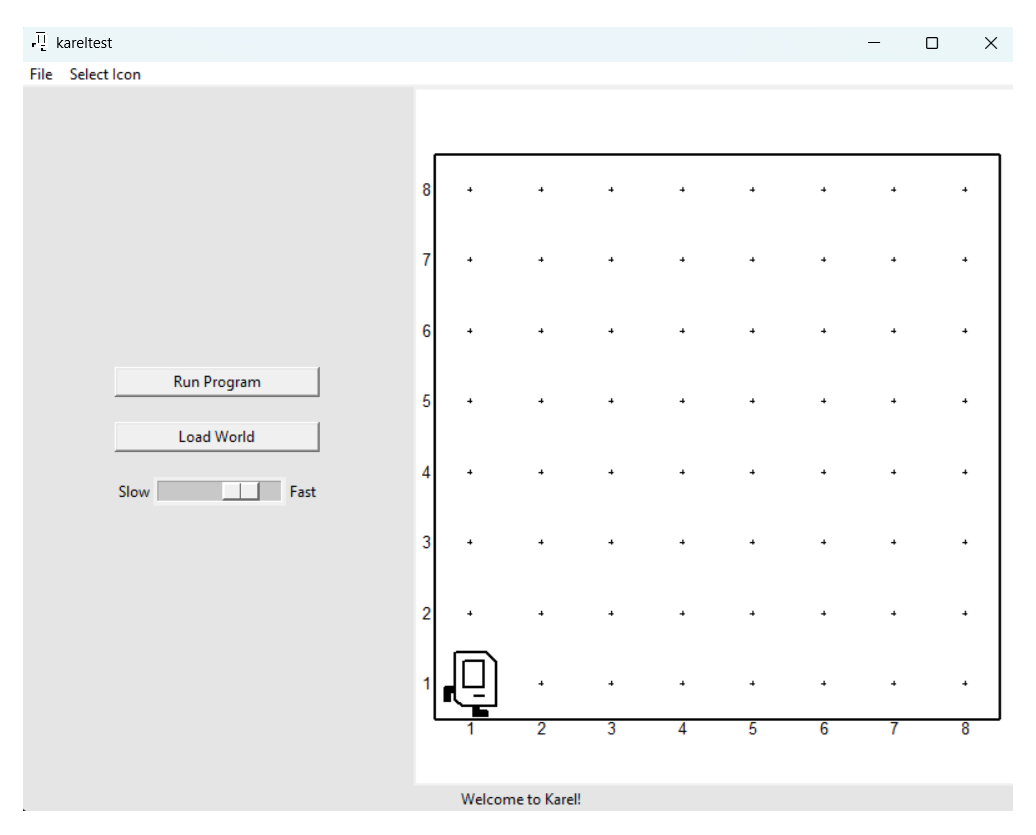
\includegraphics[scale=0.5]{Karel Window.png}
    \caption*{The Karel GUI.}
\end{figure}
In the caption above, I called this window a \textit{GUI}. You'll see that term come up all the time in programming. It stands for Graphical User Interface, and it just means that the Karel software isn't command-line based but instead has a window you can click around in. Neat!

To open a world, click ``Load World''. To run your code inside your \pythonl{main()} function, click ``Run Program.'' Try it now and see what happens!

Notice that she goes up one? That's because she turns left, which causes her to point up. Then she moves, and then she turns left, which has her pointing left. (Though in Karel the Robot, she'll always be upside down when facing left. She can still move just fine though!)

\begin{figure}[H]
    \centering
    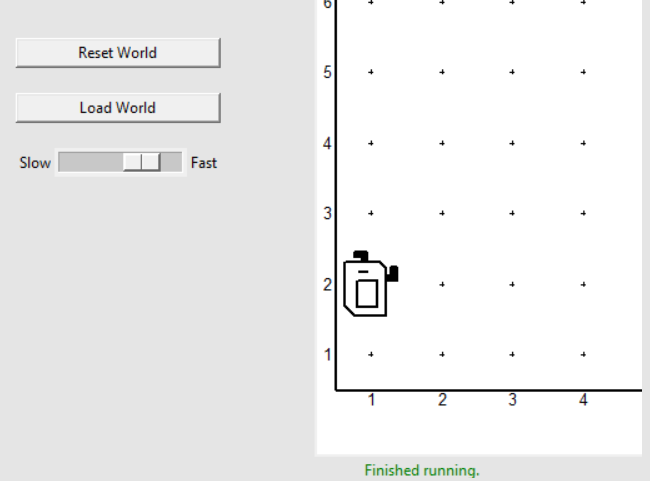
\includegraphics[scale=0.5]{Up One Face Left.png}
    \caption*{Up One, Facing Left.}
\end{figure}

Notice also that instead of writing \pythonl{move}, we write \pythonl{move()}, and instead of writing \pythonl{turn_left}, we write \pythonl{turn_left()}. This is because remember how with functions we pass in inputs through the parentheses? For example, our function \pythonl{bigger(3,5)} returned the bigger number of the two inputs. Well here, \pythonl{move()} takes in no input, so the parentheses, while still necessary, are empty. You'll get used to writing empty parentheses like \pythonl{()} a lot when programming.

\begin{center}
    \begin{minipage}{0.45\textwidth}
        \centering
        \textcolor{red}{\:Incorrect}
        \smallskip

        \pythonl{move}\\
        \pythonl{turn_left} \\
        \pythonl{pick_beeper}\\
        \pythonl{put_beeper}
    \end{minipage}
    \hfill
    \begin{minipage}{0.05\textwidth}
        \centering
        \vspace{1.8em}
        \textbf{VS}
    \end{minipage}
    \hfill
    \begin{minipage}{0.45\textwidth}
        \centering
        \textcolor{green}{Correct}
        \smallskip
        
        \pythonl{move()} \\
        \pythonl{turn_left()} \\
        \pythonl{pick_beeper()}\\
        \pythonl{put_beeper()}
    \end{minipage}
\end{center}

With the four main functions and knowledge on how to use Karel, you're ready to do some puzzles! Here's some problems I'd like you to do:

\newpage
\subsection*{Problems}
\begin{enumerate}
    \item Write code that picks up the beeper on \codel{collect_newspaper_karel.w}. You can directly launch a world without using the ``Load World'' button by changing the code to:
    
    \begin{python}
        if __name__ == "__main__":
            run_karel_program("collect_newspaper_karel")
    \end{python}

    Remember also there's a slider to control the robot's speed. For some reason it's super low when you load a world directly as I showed above, so you may want to drag it up.

    \begin{figure}
        \centering
        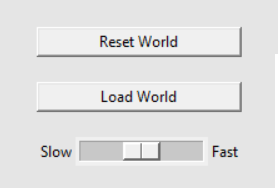
\includegraphics[scale=0.5]{SlowFast.png}
        \caption*{Pick what feels comfortable.}
    \end{figure}

    \item Write a function \pythonl{turn_around()} that turns Karel around using only\\ \pythonl{turn_left()}.
    \item Write a function \pythonl{turn_right()} that turns Karel right using only \pythonl{turn_left()}.
    \item Write a function \pythonl{turn_around_two()} that turns Karel around, but this time only uses\\ \pythonl{turn_right()} from the previous problem.
    \item Modify your code for \codel{collect_newspaper_karel.w} so that it places the beeper in the bottom left corner of the world.
\end{enumerate}






\end{document}